\documentclass{standalone}
\usepackage{tikz}
\usetikzlibrary{patterns, positioning}

\begin{document}
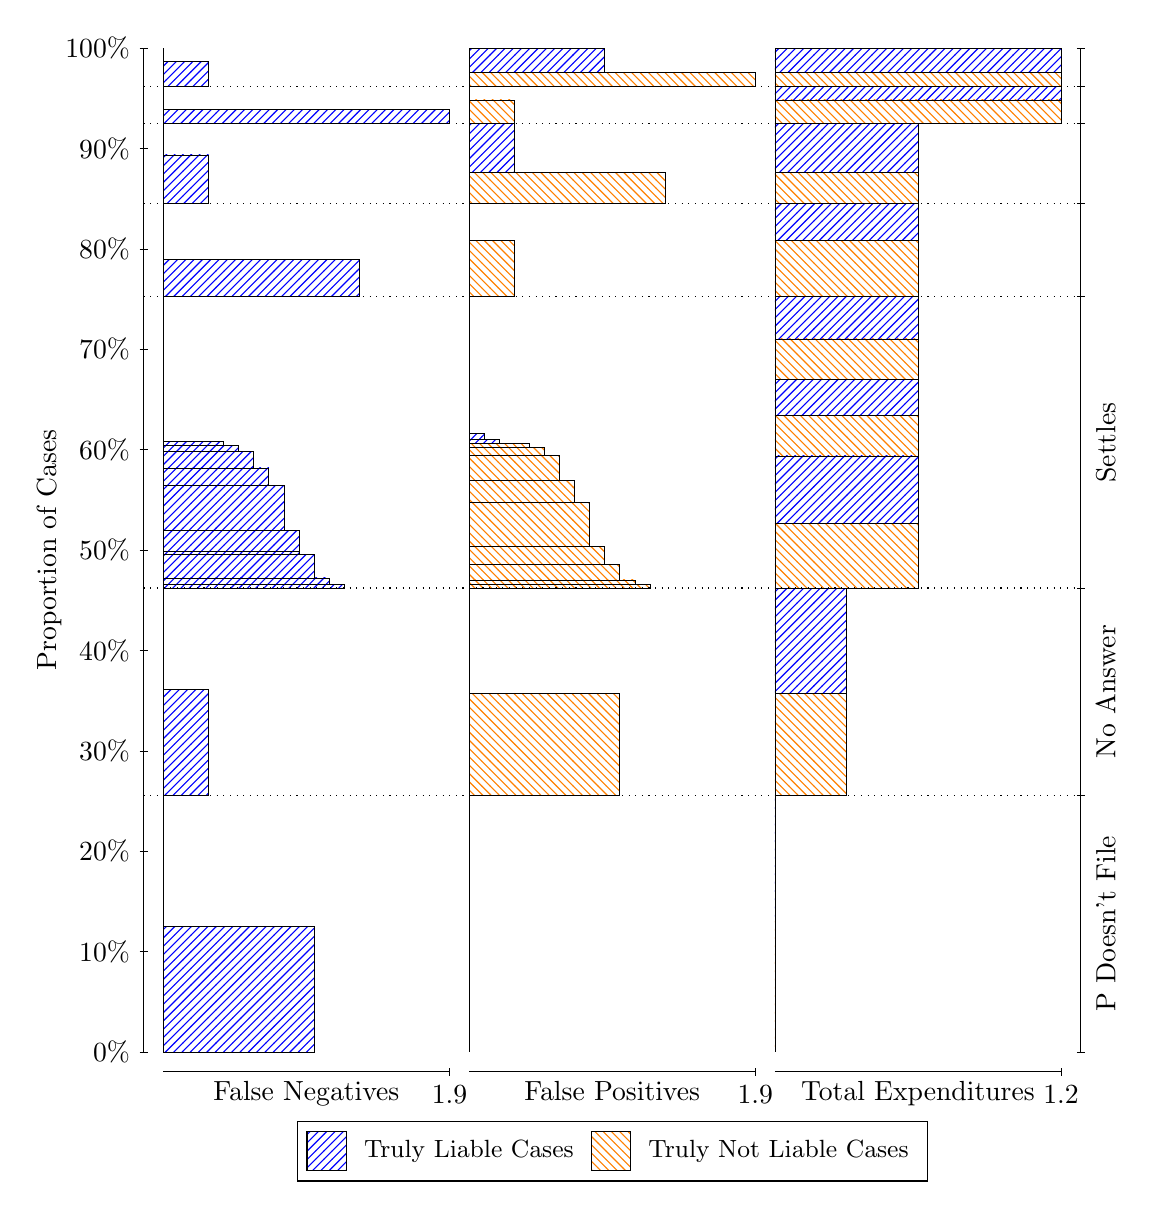
\begin{tikzpicture}
\draw[black, very thin] (1.5,1.75) -- (1.5,14.5);
\node[rotate=90, anchor=center] at (0.3, 8.125) {Proportion of Cases};
\draw[black, very thin] (1.45,1.75) -- (1.55,1.75);
\node[anchor=east] at (1.45, 1.75) {0\%};
\draw[black, very thin] (1.45,3.025) -- (1.55,3.025);
\node[anchor=east] at (1.45, 3.025) {10\%};
\draw[black, very thin] (1.45,4.3) -- (1.55,4.3);
\node[anchor=east] at (1.45, 4.3) {20\%};
\draw[black, very thin] (1.45,5.575) -- (1.55,5.575);
\node[anchor=east] at (1.45, 5.575) {30\%};
\draw[black, very thin] (1.45,6.85) -- (1.55,6.85);
\node[anchor=east] at (1.45, 6.85) {40\%};
\draw[black, very thin] (1.45,8.125) -- (1.55,8.125);
\node[anchor=east] at (1.45, 8.125) {50\%};
\draw[black, very thin] (1.45,9.4) -- (1.55,9.4);
\node[anchor=east] at (1.45, 9.4) {60\%};
\draw[black, very thin] (1.45,10.675) -- (1.55,10.675);
\node[anchor=east] at (1.45, 10.675) {70\%};
\draw[black, very thin] (1.45,11.95) -- (1.55,11.95);
\node[anchor=east] at (1.45, 11.95) {80\%};
\draw[black, very thin] (1.45,13.225) -- (1.55,13.225);
\node[anchor=east] at (1.45, 13.225) {90\%};
\draw[black, very thin] (1.45,14.5) -- (1.55,14.5);
\node[anchor=east] at (1.45, 14.5) {100\%};

\draw[black, very thin] (13.4,1.75) -- (13.4,14.5);
\draw[black, very thin] (13.35,1.75) -- (13.45,1.75);
\node[anchor=west] at (13.35, 1.75) {};
\draw[black, very thin] (13.35,5.0093) -- (13.45,5.0093);
\node[anchor=west] at (13.35, 5.0093) {};
\draw[black, very thin] (13.35,7.6422) -- (13.45,7.6422);
\node[anchor=west] at (13.35, 7.6422) {};
\draw[black, very thin] (13.35,11.341) -- (13.45,11.341);
\node[anchor=west] at (13.35, 11.341) {};
\draw[black, very thin] (13.35,12.524) -- (13.45,12.524);
\node[anchor=west] at (13.35, 12.524) {};
\draw[black, very thin] (13.35,13.542) -- (13.45,13.542);
\node[anchor=west] at (13.35, 13.542) {};
\draw[black, very thin] (13.35,14.017) -- (13.45,14.017);
\node[anchor=west] at (13.35, 14.017) {};
\draw[black, very thin] (13.35,14.5) -- (13.45,14.5);
\node[anchor=west] at (13.35, 14.5) {};

\draw[black, very thin, pattern color=blue, pattern=north east lines] (1.75,1.75) rectangle (3.6623,3.3486);
\draw[black, very thin, pattern color=orange, pattern=north west lines] (1.75,3.3486) rectangle (1.75,5.0093);
\draw[black, very thin, pattern color=blue, pattern=north east lines] (1.75,5.0093) rectangle (2.3237,6.3504);
\draw[black, very thin, pattern color=orange, pattern=north west lines] (1.75,6.3504) rectangle (1.75,7.6422);
\draw[black, very thin, pattern color=blue, pattern=north east lines] (1.75,7.6422) rectangle (4.0447,7.6908);
\draw[black, very thin, pattern color=blue, pattern=north east lines] (1.75,7.6908) rectangle (3.8535,7.7709);
\draw[black, very thin, pattern color=blue, pattern=north east lines] (1.75,7.7709) rectangle (3.6623,8.0655);
\draw[black, very thin, pattern color=blue, pattern=north east lines] (1.75,8.0655) rectangle (3.4711,8.1072);
\draw[black, very thin, pattern color=blue, pattern=north east lines] (1.75,8.1072) rectangle (3.4711,8.3738);
\draw[black, very thin, pattern color=blue, pattern=north east lines] (1.75,8.3738) rectangle (3.2798,8.9486);
\draw[black, very thin, pattern color=blue, pattern=north east lines] (1.75,8.9486) rectangle (3.0886,9.1668);
\draw[black, very thin, pattern color=blue, pattern=north east lines] (1.75,9.1668) rectangle (2.8974,9.3781);
\draw[black, very thin, pattern color=blue, pattern=north east lines] (1.75,9.3781) rectangle (2.7061,9.4521);
\draw[black, very thin, pattern color=blue, pattern=north east lines] (1.75,9.4521) rectangle (2.5149,9.5023);
\draw[black, very thin, pattern color=orange, pattern=north west lines] (1.75,9.5023) rectangle (1.75,11.341);
\draw[black, very thin, pattern color=blue, pattern=north east lines] (1.75,11.341) rectangle (4.236,11.811);
\draw[black, very thin, pattern color=orange, pattern=north west lines] (1.75,11.811) rectangle (1.75,12.524);
\draw[black, very thin, pattern color=blue, pattern=north east lines] (1.75,12.524) rectangle (2.3237,13.142);
\draw[black, very thin, pattern color=orange, pattern=north west lines] (1.75,13.142) rectangle (1.75,13.542);
\draw[black, very thin, pattern color=blue, pattern=north east lines] (1.75,13.542) rectangle (5.3833,13.719);
\draw[black, very thin, pattern color=orange, pattern=north west lines] (1.75,13.719) rectangle (1.75,14.017);
\draw[black, very thin, pattern color=blue, pattern=north east lines] (1.75,14.017) rectangle (2.3237,14.327);
\draw[black, very thin, pattern color=orange, pattern=north west lines] (1.75,14.327) rectangle (1.75,14.5);
\draw[black, very thin, pattern color=orange, pattern=north west lines] (5.6333,1.75) rectangle (5.6333,3.4107);
\draw[black, very thin, pattern color=blue, pattern=north east lines] (5.6333,3.4107) rectangle (5.6333,5.0093);
\draw[black, very thin, pattern color=orange, pattern=north west lines] (5.6333,5.0093) rectangle (7.5456,6.3011);
\draw[black, very thin, pattern color=blue, pattern=north east lines] (5.6333,6.3011) rectangle (5.6333,7.6422);
\draw[black, very thin, pattern color=orange, pattern=north west lines] (5.6333,7.6422) rectangle (7.9281,7.6854);
\draw[black, very thin, pattern color=orange, pattern=north west lines] (5.6333,7.6854) rectangle (7.7368,7.7467);
\draw[black, very thin, pattern color=orange, pattern=north west lines] (5.6333,7.7467) rectangle (7.5456,7.9467);
\draw[black, very thin, pattern color=orange, pattern=north west lines] (5.6333,7.9467) rectangle (7.3544,8.17);
\draw[black, very thin, pattern color=orange, pattern=north west lines] (5.6333,8.17) rectangle (7.1632,8.727);
\draw[black, very thin, pattern color=orange, pattern=north west lines] (5.6333,8.727) rectangle (6.9719,9.0129);
\draw[black, very thin, pattern color=orange, pattern=north west lines] (5.6333,9.0129) rectangle (6.7807,9.3289);
\draw[black, very thin, pattern color=orange, pattern=north west lines] (5.6333,9.3289) rectangle (6.5895,9.4253);
\draw[black, very thin, pattern color=orange, pattern=north west lines] (5.6333,9.4253) rectangle (6.3982,9.4806);
\draw[black, very thin, pattern color=blue, pattern=north east lines] (5.6333,9.4806) rectangle (6.0158,9.5307);
\draw[black, very thin, pattern color=blue, pattern=north east lines] (5.6333,9.5307) rectangle (5.8246,9.6048);
\draw[black, very thin, pattern color=blue, pattern=north east lines] (5.6333,9.6048) rectangle (5.6333,11.341);
\draw[black, very thin, pattern color=orange, pattern=north west lines] (5.6333,11.341) rectangle (6.207,12.054);
\draw[black, very thin, pattern color=blue, pattern=north east lines] (5.6333,12.054) rectangle (5.6333,12.524);
\draw[black, very thin, pattern color=orange, pattern=north west lines] (5.6333,12.524) rectangle (8.1193,12.924);
\draw[black, very thin, pattern color=blue, pattern=north east lines] (5.6333,12.924) rectangle (6.207,13.542);
\draw[black, very thin, pattern color=orange, pattern=north west lines] (5.6333,13.542) rectangle (6.207,13.84);
\draw[black, very thin, pattern color=blue, pattern=north east lines] (5.6333,13.84) rectangle (5.6333,14.017);
\draw[black, very thin, pattern color=orange, pattern=north west lines] (5.6333,14.017) rectangle (9.2667,14.19);
\draw[black, very thin, pattern color=blue, pattern=north east lines] (5.6333,14.19) rectangle (7.3544,14.5);
\draw[black, very thin, pattern color=orange, pattern=north west lines] (9.5167,1.75) rectangle (9.5167,3.4107);
\draw[black, very thin, pattern color=blue, pattern=north east lines] (9.5167,3.4107) rectangle (9.5167,5.0093);
\draw[black, very thin, pattern color=orange, pattern=north west lines] (9.5167,5.0093) rectangle (10.425,6.3011);
\draw[black, very thin, pattern color=blue, pattern=north east lines] (9.5167,6.3011) rectangle (10.425,7.6422);
\draw[black, very thin, pattern color=orange, pattern=north west lines] (9.5167,7.6422) rectangle (11.333,8.4605);
\draw[black, very thin, pattern color=blue, pattern=north east lines] (9.5167,8.4605) rectangle (11.333,9.3206);
\draw[black, very thin, pattern color=orange, pattern=north west lines] (9.5167,9.3206) rectangle (11.333,9.8307);
\draw[black, very thin, pattern color=blue, pattern=north east lines] (9.5167,9.8307) rectangle (11.333,10.296);
\draw[black, very thin, pattern color=orange, pattern=north west lines] (9.5167,10.296) rectangle (11.333,10.806);
\draw[black, very thin, pattern color=blue, pattern=north east lines] (9.5167,10.806) rectangle (11.333,11.341);
\draw[black, very thin, pattern color=orange, pattern=north west lines] (9.5167,11.341) rectangle (11.333,12.054);
\draw[black, very thin, pattern color=blue, pattern=north east lines] (9.5167,12.054) rectangle (11.333,12.524);
\draw[black, very thin, pattern color=orange, pattern=north west lines] (9.5167,12.524) rectangle (11.333,12.924);
\draw[black, very thin, pattern color=blue, pattern=north east lines] (9.5167,12.924) rectangle (11.333,13.542);
\draw[black, very thin, pattern color=orange, pattern=north west lines] (9.5167,13.542) rectangle (13.15,13.84);
\draw[black, very thin, pattern color=blue, pattern=north east lines] (9.5167,13.84) rectangle (13.15,14.017);
\draw[black, very thin, pattern color=orange, pattern=north west lines] (9.5167,14.017) rectangle (13.15,14.19);
\draw[black, very thin, pattern color=blue, pattern=north east lines] (9.5167,14.19) rectangle (13.15,14.5);
\draw[black, dotted] (1.5,5.0093) -- (13.4,5.0093);
\draw[black, dotted] (1.5,7.6422) -- (13.4,7.6422);
\draw[black, dotted] (1.5,11.341) -- (13.4,11.341);
\draw[black, dotted] (1.5,12.524) -- (13.4,12.524);
\draw[black, dotted] (1.5,13.542) -- (13.4,13.542);
\draw[black, dotted] (1.5,14.017) -- (13.4,14.017);
\draw[black, very thin] (1.75,1.5) -- (5.3833,1.5);
\node[anchor=north] at (3.5667, 1.5) {False Negatives};
\draw[black, very thin] (5.3833,1.45) -- (5.3833,1.55);
\node[anchor=north] at (5.3833, 1.45) {1.9};

\draw[black, very thin] (5.6333,1.5) -- (9.2667,1.5);
\node[anchor=north] at (7.45, 1.5) {False Positives};
\draw[black, very thin] (9.2667,1.45) -- (9.2667,1.55);
\node[anchor=north] at (9.2667, 1.45) {1.9};

\draw[black, very thin] (9.5167,1.5) -- (13.15,1.5);
\node[anchor=north] at (11.333, 1.5) {Total Expenditures};
\draw[black, very thin] (13.15,1.45) -- (13.15,1.55);
\node[anchor=north] at (13.15, 1.45) {1.2};

\node[black, centered, rotate=90] at (13.72, 3.3797) {P Doesn't File};
\node[black, centered, rotate=90] at (13.72, 6.3258) {No Answer};
\node[black, centered, rotate=90] at (13.72, 9.4914) {Settles};





\draw (7.449999999999999,1.5) node[draw=none] (baseCoordinate) {};
\begin{scope}[align=center]
        \matrix[scale=0.5, draw=black, below=0.5cm of baseCoordinate, nodes={draw}, column sep=0.1cm]{
            \node[rectangle, draw, minimum width=0.5cm, minimum height=0.5cm, pattern=north east lines, pattern color=blue] {}; &
            \node[draw=none, font=\small] (B) {Truly Liable Cases}; &
            \node[rectangle, draw, minimum width=0.5cm, minimum height=0.5cm, pattern=north west lines, pattern color=orange] {}; &
            \node[draw=none, font=\small] (B) {Truly Not Liable Cases}; \\
            };
\end{scope}

\end{tikzpicture}
\end{document}